\documentclass[journal]{IEEEtran}
\usepackage[a5paper, margin=10mm, onecolumn]{geometry}
\usepackage{lmodern} % Ensure lmodern is loaded for pdflatex
\usepackage{tfrupee} % Include tfrupee package
\usepackage{booktabs}
\setlength{\headheight}{1cm} % Set the height of the header box
\setlength{\headsep}{0mm}  % Set the distance between the header box and the top of the text

\usepackage{csquotes}
\usepackage{gvv-book}
\usepackage{gvv}
\usepackage{circuitikz}
\usepackage{cite}
\usepackage{amsmath,amssymb,amsfonts,amsthm}
\usepackage{algorithmic}
\usepackage{graphicx}
\usepackage{textcomp}
\usepackage{xcolor}
\usepackage{txfonts}
\usepackage{listings}
\usepackage{enumitem}
\usepackage{mathtools}
\usepackage{gensymb}
\usepackage{comment}
\usepackage[breaklinks=true]{hyperref}
\usepackage{tkz-euclide} 
\usepackage{listings}
% \usepackage{gvv}                                        
\def\inputGnumericTable{}                                 
\usepackage[latin1]{inputenc}                                
\usepackage{color}                                            
\usepackage{array}                                            
\usepackage{longtable}                                       
\usepackage{calc}                                             
\usepackage{multirow}                                         
\usepackage{hhline}                                           
\usepackage{ifthen}                                           
\usepackage{lscape}
\usepackage{caption}
\usepackage{tikz}
\usetikzlibrary{patterns}
\begin{document}

\bibliographystyle{IEEEtran}

\begin{center}
    \textbf{\Large GATE 2020\\
    AGRICULTURAL ENGINEERING (AG)\\
    MAIN PAPER}
\end{center}

\section*{GA - General Aptitude}

\textbf{Q1 -- Q5 carry one mark each.}

\begin{enumerate}
\item 
The untimely loss of life is a cause of serious global concern as thousands of people get killed\dots accidents every year while many other die\dots diseases like cardio vascular disease, cancer, etc.

\begin{enumerate}
\begin{multicols}{2}
\item in, of
\item from, of
\item during, from
\item from, from
\end{multicols}
\end{enumerate}
\hfill(GATE AG 2020)\\

\medskip

\item 
He was not only accused of theft\dots of conspiracy.

\begin{enumerate}
\begin{multicols}{2}
\item rather
\item but also
\item but even
\item rather than
\end{multicols}
\end{enumerate}
\hfill(GATE AG 2020)\\

\medskip

\item 
Select the word that fits the analogy:

Explicit: Implicit :: Express: \dots

\begin{enumerate}
\begin{multicols}{2}
\item Impress
\item Repress
\item Compress
\item Suppress
\end{multicols}
\end{enumerate}
\hfill(GATE AG 2020)\\

\medskip

\item 
The Canadian constitution requires that equal importance be given to English and French. Last year, Air Canada lost a lawsuit, and had to pay a six-figure fine to a French-speaking couple after they filed complaints about formal in-flight announcements in English lasting 15 seconds, as opposed to informal 5 second messages in French.

The French-speaking couple were upset at \dots.

\begin{enumerate}
\begin{multicols}{2}
\item the in-flight announcements being made in English.
\item the English announcements being clearer than the French ones.
\item the English announcements being longer than the French ones.
\item equal importance being given to English and French.
\end{multicols}
\end{enumerate}
\hfill(GATE AG 2020)\\

\medskip

\item 
A superadditive function $f(\cdot)$ satisfies the following property
\begin{align*}
f(x_1 + x_2) \geq f(x_1) + f(x_2)
\end{align*}
Which of the following functions is a superadditive function for $x > 1$?
\begin{enumerate}
\begin{multicols}{2}
\item $e^x$
\item $\sqrt{x}$
\item $\frac{1}{x}$
\item $e^{-x}$
\end{multicols}
\end{enumerate}
\hfill(GATE AG 2020)\\

\medskip

\item 
The global financial crisis in 2008 is considered to be the most serious world-wide financial crisis, which started with the sub-prime lending crisis in USA in 2007. The sub-prime lending crisis led to the banking crisis in 2008 with the collapse of Lehman Brothers in 2008. The sub-prime lending refers to the provision of loans to those borrowers who may have difficulties in repaying loans, and it arises because of excess liquidity following the East Asian crisis.

Which one of the following sequences shows the correct precedence as per the given passage?
\begin{enumerate}
\begin{multicols}{2}
\item East Asian crisis $\to$ subprime lending crisis $\to$ banking crisis $\to$ global financial crisis.
\item Subprime lending crisis $\to$ global financial crisis $\to$ banking crisis $\to$ East Asian crisis.
\item Banking crisis $\to$ subprime lending crisis $\to$ global financial crisis $\to$ East Asian crisis.
\item Global financial crisis $\to$ East Asian crisis $\to$ banking crisis $\to$ subprime lending crisis.
\end{multicols}
\end{enumerate}
\hfill(GATE AG 2020)\\

\medskip

\item 
It is quarter past three in your watch. The angle between the hour hand and the minute hand is\dots.

\begin{enumerate}
\begin{multicols}{2}
\item $0^\circ$
\item $7.5^\circ$
\item $15^\circ$
\item $22.5^\circ$
\end{multicols}
\end{enumerate}
\hfill(GATE AG 2020)\\

\medskip

\item 
A circle with centre O is shown in the figure. A rectangle PQRS of maximum possible area is inscribed in the circle. If the radius of the circle is $a$, then the area of the shaded portion is\dots.

\begin{figure}[h]
    \centering
    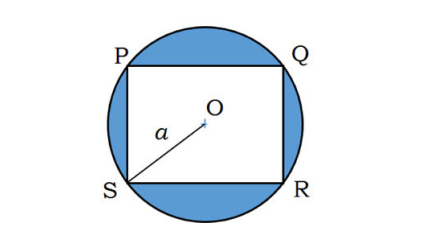
\includegraphics[width=0.7\columnwidth]{Figs/Screenshot 2025-08-24 152216.png}
    \caption{}
    \label{fig 1}
\end{figure}

\begin{enumerate}
\begin{multicols}{2}
\item $\pi a^2 - a^2$
\item $\pi a^2 - \sqrt{2}a^2$
\item $\pi a^2 - 2a^2$
\item $\pi a^2 - 3a^2$
\end{multicols}
\end{enumerate}
\hfill(GATE AG 2020)\\

\medskip

\item 
$a, b, c$ are real numbers. The quadratic equation $a x^2 - b x + c = 0$ has equal roots, which is $\beta$, then
\begin{enumerate}
\begin{multicols}{2}
\item $\beta = b/a$
\item $\beta^2 = ac$
\item $\beta^3 = \frac{bc}{2a^2}$
\item $b^2 \neq 4ac$
\end{multicols}
\end{enumerate}
\hfill(GATE AG 2020)\\

\medskip

\item 
The following figure shows the data of students enrolled in 5 years (2014 to 2018) for two schools P and Q. During this period, the ratio of the average number of the students enrolled in school P to the average of the difference of the number of students enrolled in schools P and Q is\dots.

\begin{figure}[h]
    \centering
    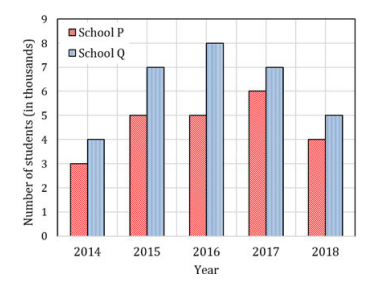
\includegraphics[width=0.7\columnwidth]{Figs/Screenshot 2025-08-24 152447.png}
    \caption{}
    \label{fig 2}
\end{figure}

\begin{enumerate}
\begin{multicols}{2}
\item $8 : 23$
\item $23 : 8$
\item $23 : 31$
\item $31 : 23$
\end{multicols}
\end{enumerate}
\hfill(GATE AG 2020)\\

\medskip

\item 
The function $f(x) = x^4 - 4x^3 + 6x^2 - 4x + 1$ has a
\begin{enumerate}
\begin{multicols}{2}
\item Maxima at $x = 0$
\item Minima at $x = 0$
\item Maxima at $x = 1$
\item Minima at $x = 1$
\end{multicols}
\end{enumerate}
\hfill(GATE AG 2020)\\

\medskip

\item 
A linear system of equations has $n$ unknowns. The ranks of the coefficient matrix and the augmented matrix of the linear system of equations are $r_1$ and $r_2$, respectively. The condition for the equations to be consistent with a unique solution is
\begin{enumerate}
\begin{multicols}{2}
\item $r_1 \neq r_2 < n$
\item $r_1 = r_2 = n$
\item $r_1 = r_2 < n$
\item $r_1 \neq r_2 > n$
\end{multicols}
\end{enumerate}
\hfill(GATE AG 2020)\\

\medskip

\item 
General solution to the ordinary differential equation,
\begin{align*}
\frac{d^3y}{dx^3} - 6 \frac{d^2y}{dx^2} + 11 \frac{dy}{dx} - 6y = 0
\end{align*}
is
\begin{enumerate}
\begin{multicols}{2}
\item $C_1 e^x + C_2 e^{2x} + C_3 e^{3x}$
\item $C_1 e^x + C_2 e^{2x} + C_3 e^x$
\item $C_1 e^x + C_2 e^{2x} + C_3 e^{3x}$
\item $C_1 e^x + C_2 e^{2x} + C_3 e^{3x}$
\end{multicols}
\end{enumerate}
\hfill(GATE AG 2020)\\

\medskip

\item 
In a tractor steering system, the angle made by the kingpin axis projected on the longitudinal plane of the tractor with the vertical axis is known as
\begin{enumerate}
\begin{multicols}{2}
\item Kingpin inclination
\item Caster angle
\item Camber angle
\item Steering angle
\end{multicols}
\end{enumerate}
\hfill(GATE AG 2020)\\

\medskip

\item 
A tractor operated 9-row precision planter has 16 cells on the metering plates. The speed ratio of the metering plates to the ground drive wheel is 1:2 and the rolling diameter of the ground drive wheel is 40 cm. Assuming no skid, the plant to plant spacing in rows in \textbf{mm} is
\begin{enumerate}
\begin{multicols}{2}
\item 39
\item 50
\item 157
\item 314
\end{multicols}
\end{enumerate}
\hfill(GATE AG 2020)\\

\medskip

\item 
A self-propelled wheel does not have
\begin{enumerate}
\begin{multicols}{2}
\item Wheel torque
\item Tractive power
\item Rolling resistance
\item Drawbar pull
\end{multicols}
\end{enumerate}
\hfill(GATE AG 2020)\\

\medskip

\item 
Match the following items between Column I and Column II with the most appropriate combinations:

\begin{tabular}{>{\bfseries}l l}
Specification & Outer Diameter in mm \\
P. AW & p. 34.9 \\
Q. BW & q. 44.4 \\
R. EW & r. 54.0 \\
S. NW & s. 66.7 \\
\end{tabular}



\begin{enumerate}
\begin{multicols}{2}
\item P-3, Q-2, R-1, S-4
\item P-2, Q-3, R-1, S-4
\item P-2, Q-3, R-4, S-1
\item P-3, Q-2, R-4, S-1
\end{multicols}
\end{enumerate}
\hfill(GATE AG 2020)\\

\medskip

\item 
From the performance evaluation of drippers, the discharge exponent value and the coefficient of variation were obtained as 0.5 and 0.04, respectively. The drippers are categorized as
\begin{enumerate}
\begin{multicols}{2}
\item Pressure compensating drippers of excellent quality
\item Turbulent flow-tortuous path orifice type drippers of good quality
\item Turbulent flow-tortuous path orifice type drippers of marginal quality
\item Laminar flow drippers of excellent quality
\end{multicols}
\end{enumerate}
\hfill(GATE AG 2020)\\

\medskip

\item 
In a basin, rainfall is recorded by five automatic weather stations A, B, C, D and E with respective average annual rainfall of 1020, 810, 675, 940 and 780 mm. In a particular year, the station A was non-operational and the remaining stations B, C, D and E recorded annual rainfall of 890, 725, 980 and 850 mm, respectively. The estimated rainfall at the station A in that particular year in \textbf{mm} is
\begin{enumerate}
\begin{multicols}{2}
\item 758
\item 878
\item 1038
\item 1098
\end{multicols}
\end{enumerate}
\hfill(GATE AG 2020)\\

\medskip

\item 
A field crop is irrigated when the available soil water reduces to 60\%. The moisture content at field capacity and wilting point are 32\% and 12\%, respectively. The bulk density of the soil is 1.5 g cm$^{-3}$. The field water application efficiency is 75\% and the crop root zone depth is 50 cm. The gross depth of irrigation required to bring soil moisture content to field capacity in \textbf{cm} is
\begin{enumerate}
\begin{multicols}{2}
\item 6
\item 8
\item 9
\item 12
\end{multicols}
\end{enumerate}
\hfill(GATE AG 2020)\\

\medskip

\item 
A cold storage takes 5 hours to bring down the temperature of 100 metric tons of potato from 35$^\circ$C to 8$^\circ$C. The specific heat capacity of potato is 3.1 kJ kg$^{-1}$ $^\circ$C$^{-1}$. The coefficient of performance (COP) and the latent heat of vaporisation of the refrigerant (R-22) at an evaporation temperature of $-$10$^\circ$C are 3.66 and 230 kJ kg$^{-1}$, respectively. Neglecting respiration heat load of potato, and assuming no power loss, the values of refrigerant flow rate and the power input to the compressor are
\begin{enumerate}
\begin{multicols}{2}
\item 121.3 kg min$^{-1}$ and 127.1 kW
\item 124.7 kg min$^{-1}$ and 121.3 kW
\item 127.1 kg min$^{-1}$ and 121.3 kW
\item 124.7 kg min$^{-1}$ and 127.1 kW
\end{multicols}
\end{enumerate}
\hfill(GATE AG 2020)\\

\medskip

\item 
Hydrothermal treatment of paddy makes
\begin{enumerate}
\begin{multicols}{2}
\item Shelling more difficult
\item Polishing of parboiled rice easier
\item Higher retention of vitamins and minerals
\item Kernel soft, resulting in faster cooking
\end{multicols}
\end{enumerate}
\hfill(GATE AG 2020)\\

\medskip

\item 
Both particle formation and drying process are carried out by
\begin{enumerate}
\begin{multicols}{2}
\item Flash dryer
\item Fluidized bed dryer
\item Pneumatic conveyor dryer
\item Spray dryer
\end{multicols}
\end{enumerate}
\hfill(GATE AG 2020)\\

\medskip

\item 
If one of the two Eigenvalues of a matrix
$\myvec{ 3 & 2 \\ 2 & 1 }$ is 4.236, then the other Eigenvalue (\textit{round off to 3 decimal places}) is \dots.

\begin{align*}
\lim_{x \to 0} \frac{e^{x} - e^{-x} - 2x}{x - \sin x}
\end{align*}
is \dots.
\hfill(GATE AG 2020)\\

\medskip


\item 
At the maximum power output of a solar panel, the voltage and current are 18 V and 5.56 A, respectively. If the open circuit voltage and short circuit current of the same solar panel are 21.6 V and 6.11 A, respectively, the fill factor of the panel (\textit{round off to 2 decimal places}) is \dots.
\hfill(GATE AG 2020)\\

\medskip

\item 
The sound pressure level on the operator's seat of a tractor is 80 dB. If the reference sound pressure is $2 \times 10^{-5}$ N m$^{-2}$, the root mean square (RMS) sound pressure in N m$^{-2}$ (\textit{round off to 2 decimal places}) is \dots.
\hfill(GATE AG 2020)\\

\medskip

\item 
A towed pneumatic wheel with an unloaded radius of 330 mm covers a distance of 9.9 m in 5 revolutions without any skid. Assuming the rolling radius to be same as the static loaded radius of the wheel, the deflection of the wheel in \textbf{mm} (\textit{round off to 1 decimal place}) is \dots.
\hfill(GATE AG 2020)\\

\medskip

\item 
The grain to straw ratio of 500 kg feed material is 3:2. The blown grain loss, separation loss and cleaning efficiency of the thresher are 0.05\%, 0.5\% and 99.1\%, respectively. Considering 100\% threshing efficiency, grain recovery at the main grain outlet in \textbf{kg} (\textit{round off to 2 decimal places}) is \dots.
\hfill(GATE AG 2020)\\

\medskip

\item 
A tubewell has a discharge of 40 m$^3$ h$^{-1}$ and operates daily for 20 h during irrigation season. The irrigation interval is 20 days and depth of irrigation is 8 cm. The command area of tubewell in \textbf{ha} is \dots.
\hfill(GATE AG 2020)\\

\medskip

\item 
The drainage coefficient of a watershed of 720 ha area is 1.2 cm. The design discharge of the drain in \textbf{m$^3$ s$^{-1}$} is \dots.
\hfill(GATE AG 2020)\\

\medskip

\item 
The following data were used for a watershed experiencing soil erosion problem:

Rainfall Erosivity Index = 280 MJ mm ha$^{-1}$ h$^{-1}$ year$^{-1}$, \\
Soil Erodibility Index = 0.38 ton ha h MJ$^{-1}$ mm$^{-1}$, \\
Slope length = 200 m, Average slope of the land = 8\%, \\
Slope steepness factor = 0.85, Cropping management factor = 0.35, Conservation practice factor = 0.60.

If the slope length is reduced to half, \textbf{percentage} reduction in soil loss (\textit{round off to 2 decimal places}) is \dots.
\hfill(GATE AG 2020)\\

\medskip

\item 
Fresh tomato juice containing 6\% (w/w) total solids enters in a single effect evaporator at a feed rate of 500 kg h$^{-1}$ to concentrate up to 36\% (w/w) solids. In this process, the rate of water removal in \textbf{kg h$^{-1}$} (\textit{round off to 1 decimal place}) is \dots.
\hfill(GATE AG 2020)\\

\medskip

\item
Heat gain is occurring through a composite cold storage wall, made of brick and polyurethane foam insulation (thickness and thermal conductivity values are given below). If the exposed surfaces of brick and insulation are at $45~^\circ\mathrm{C}$ and $10~^\circ\mathrm{C}$, respectively, the temperature at the interface of brick and insulation in $^\circ\mathrm{C}$ \textit{(round off to 1 decimal place)} is \dots.
\hfill(GATE AG 2020)\\

\begin{center}
\begin{tabular}{|c|c|c|c|c|c|}
\hline
Mass of particles, g      & 2   & 5   & 7   & 4   & 1    \\
\hline
Mean size of particles, $\mu$m & 350 & 240 & 200 & 150 & 100 \\
\hline
\end{tabular}
\end{center}

\medskip

\item 
A milk processing plant pasteurizes a batch of 12500 L whole milk to inactivate the pathogen \textit{Coxiella burnetii}, (decimal reduction time of 14 seconds at 72~$^\circ$C) prior to packing in 500 milliliter pouches. The initial count of the noted organism is 10 per milliliter. For this batch pasteurization process at 72~$^\circ$C, resulting in no survivor in any of the packages, the process F-value in \textbf{seconds} is \dots.
\hfill(GATE AG 2020)\\

\medskip

\item 
A particle moves along the curve 
\begin{align*}
\vec{R} = (2t^3 + 4t^2)\,\hat{\imath} + (3t^2 - 5t)\,\hat{\jmath} + (7t^2 + 6t)\,\hat{k},
\end{align*} 
where $t$ is the time. The velocity component of the particle in the direction $3\,\hat{\imath} + 2\,\hat{\jmath} + \hat{k}$ at time $t = 2$ is

\begin{enumerate}
\begin{multicols}{2}
\item $\frac{122}{\sqrt{14}}$
\item $122$
\item $\frac{168}{\sqrt{14}}$
\item $168$
\end{multicols}
\end{enumerate}
\hfill(GATE AG 2020)\\

\medskip

\item 
Let a function $f(t) = 4\cos{2t} + 6e^{-8t}$. The Laplace transform of the given function $f(t)$, $\mathcal{L}\{f(t)\} = F(s) = \int_0^\infty f(t)e^{-st}dt$ is

\begin{enumerate}
\begin{multicols}{2}
\item $\frac{4s}{s^2+4} + \frac{6}{s+8}$
\item $\frac{8}{s^2+4} + \frac{6}{s-8}$
\item $\frac{4s}{s^2-4} + \frac{6}{s-8}$
\item $\frac{8}{s^2-4} + \frac{6}{s-8}$
\end{multicols}
\end{enumerate}
\hfill(GATE AG 2020)\\

\medskip

\item 
In an irrigation channel of uniform section, water passes through a $90^\circ$ triangular weir measuring 36~cm head over the crest. After traveling certain distance in the same channel, water passes through 1.0~m long rectangular weir. There is no loss of water in between two weirs. Using Francis' formula, the head over the crest of rectangular weir in \textbf{cm} is

\begin{enumerate}
\begin{multicols}{2}
\item 22.1
\item 18.4
\item 15.0
\item 11.8
\end{multicols}
\end{enumerate}
\hfill(GATE AG 2020)\\

\medskip

\item
Two ends of a differential mercury manometer are connected at two points on a pipe carrying oil. The manometer shows difference in mercury level of 20 cm. The specific gravity of oil and mercury are 0.8 and 13.6, respectively. The density of water is 1000 kg/m\textsuperscript{3} at 4\textdegree C and acceleration due to gravity ($g$) is 9.81 m/s\textsuperscript{2}.\\
At the same two points in pipe, the difference of pressure in N m\textsuperscript{2} is

\begin{enumerate}
\begin{multicols}{2}
\item 25.11
\item 251.14
\item 25113.60
\item 251136.00
\end{multicols}
\end{enumerate}
\hfill(GATE AG 2020)\\

\medskip

\item
Match the following items between Column I and Column II with the most appropriate combinations:

\begin{table}[ht]
\centering
\begin{tabular}{|l|l|}
\hline
\textbf{Column I} & \textbf{Column II} \\ \hline
P. Hydraulic Conductivity   & 1. Upper limit of moisture available to plant \\ \hline
Q. Permeability            & 2. All soil pores are filled with water         \\ \hline
R. Viscosity               & 3. Soil capillarity                            \\ \hline
S. Surface Tension         & 4. Properties of fluid as well as soil          \\ \hline
T. Saturation Capacity     & 5. Property of the medium                      \\ \hline
U. Field Capacity          & 6. Internal friction that brings about resistance to flow \\ \hline
\end{tabular}
\end{table}

\noindent
\textbf{Options:}
\begin{enumerate}
\begin{multicols}{2}
\item P-4, Q-5, R-6, S-3, T-1, U-2
\item P-5, Q-4, R-6, S-3, T-2, U-1
\item P-4, Q-5, R-3, S-6, T-2, U-1
\item P-5, Q-6, R-3, S-3, T-2, U-1
\end{multicols}
\end{enumerate}
\hfill(GATE AG 2020)\\

\medskip

\item
A retaining wall of 5 m height retains cohesionless dry soil having density of \(1.9\) Mg~m\(^{-3}\) and angle of internal friction of \(28^\circ\).
The surface of the backfill soil is horizontal.
The active and passive earth pressures per meter length of the wall in \textbf{kN} are\dots and\dots, respectively. 
\textnormal{[Take \(g = 9.81~\mathrm{m~s^{-2}}\)]}

\begin{enumerate}
\begin{multicols}{2}
\item 84.11, 645.38
\item 645.38, 84.11
\item 142.12, 381.63
\item 381.63, 142.12
\end{multicols}
\end{enumerate}
\hfill(GATE AG 2020)\\

\medskip

\item
A 40 cm diameter tubewell is constructed in a 10 m thick confined aquifer having hydraulic conductivity of \(25~\mathrm{m~day}^{-1}\). The piezometric surface is observed to be 40 m high from the impervious stratum at the radius of influence of 500 m. 
The drawdown in the tubewell is 30 m. If the thickness of aquifer is doubled and diameter of tubewell is reduced to half, keeping all other parameters and conditions same, the change in discharge from the well is \dots
\textnormal{[Take $pi = 3.14$]}

\begin{enumerate}
\begin{multicols}{2}
\item Increased by 83.72\%
\item Decreased by 83.72\%
\item Increased by 82.28\%
\item Decreased by 82.28\%
\end{multicols}
\end{enumerate}
\hfill(GATE AG 2020)\\

\medskip

\item
Choose the correct combination of process (Column I) performed by corresponding machine component(s) (Column II):

\begin{center}
\begin{tabular}{|c|c|c|c|c|c|c|}
\hline
\textbf{S. No.} & 1 & 2 & 3 & 4 & 5 & 6 \\
\hline
\textbf{H/W (mm/kg)} & 23.9 & 23.7 & 21.3 & 22.1 & 25.3 & 23.3 \\
\hline
\end{tabular}
\end{center}

\begin{enumerate}
\begin{multicols}{2}
\item P-4, Q-1, R-3, S-2
\item P-4, Q-3, R-1, S-2
\item P-1, Q-4, R-3, S-2
\item P-2, Q-1, R-4, S-3
\end{multicols}
\end{enumerate}
\hfill(GATE AG 2020)\\

\medskip

\item
Saturated steam at 121~$^\circ$C is used to sterilize pineapple juice by direct steam injection. The initial temperature of the juice is 80~$^\circ$C and after sterilization, the blend of diluted juice exits the sterilizer at 95~$^\circ$C. The enthalpy values of steam and condensate water are given in Table below. Specific heat capacity of the juice is 3.9~kJ~kg$^{-1}$~$^\circ$C$^{-1}$. Assuming no energy loss to the surroundings in the process of sterilization, the ratio of juice sterilized to steam utilized is

\begin{center}
\begin{tabular}{|l|c|c|}
\hline
Description & \textbf{P} & \textbf{Q} \\
\hline
R.L. of the ground surface, m & 220 & 220 \\
Depth of piezometer, m & 60 & 50 \\
Depth to groundwater level from ground surface, m & 60 & 50 \\
\hline
\end{tabular}
\end{center}

\begin{enumerate}
\begin{multicols}{2}
\item 34.79
\item 37.94
\item 39.47
\item 43.97
\end{multicols}
\end{enumerate}
\hfill(GATE AG 2020)\\

\medskip

\item
Hot refined oil at $120~^\circ\mathrm{C}$ enters a concentric tube-in-tube heat exchanger (HE) at the rate of $20~\mathrm{kg~min^{-1}}$. The oil is cooled by water entering at a temperature of $30~^\circ\mathrm{C}$ from the other end of the HE at the rate of $50~\mathrm{kg~min^{-1}}$. Specific heat capacities of oil and water are $1.9$ and $4.2~\mathrm{kJ~kg^{-1}~^\circ C^{-1}}$, respectively. The effectiveness of the HE may be taken as $0.7$. Assuming no heat loss to the surrounding under steady-state condition, the exit temperature of water from the HE in $^\circ$C is
\begin{enumerate}
\begin{multicols}{2}
\item 39.9
\item 41.4
\item 57.7
\item 63.0
\end{multicols}
\end{enumerate}
\hfill(GATE AG 2020)\\

\medskip

\item 
Taking six intervals, each of $\pi/12$ and using Simpson's one-third rule, the value of the definite integral $\int_{0}^{\pi/3} \sqrt{\cos \theta} ~d\theta$ \emph{(round off to 3 decimal places)} is\dots.
\hfill(GATE AG 2020)\\

\medskip

\item 
Two playing cards are drawn at random, but in succession from a pack of red cards (26 in number) without replacement. The probability of drawing a king first, followed by drawing a queen is $P \approx 10^{-3}$. The value of $P$ \emph{(round off to 3 decimal places)} is\dots.
\hfill(GATE AG 2020)\\

\medskip

\item 
A hydraulic sprayer when operating at a speed of $10~\mathrm{km~h^{-1}}$ and working pressure of $420~\mathrm{kPa}$ covers a width of $4.5~\mathrm{m}$. The power requirement and efficiency of the pump are $0.75~\mathrm{kW}$ and $70\%$, respectively. Out of total pump discharge, $10\%$ is bypassed for agitation purpose. The working pressure is increased to $500~\mathrm{kPa}$. Assuming no change in the width of coverage, the application rate of the sprayer in $\mathrm{L~ha^{-1}}$ \emph{(round off to 1 decimal place)} is\dots.
\hfill(GATE AG 2020)\\

\medskip

\item 
A tractor PTO operated rotary disc mower has 4 rotating discs and the width of cut of each disc is $60~\mathrm{cm}$ without any overlap. The specific power losses to air, stubble and gear-train friction is $2.5~\mathrm{kW}$ per meter of cutting width. The specific cutting energy requirement is $2.0~\mathrm{kJ~m^{-2}}$. If the machine is operated at a forward speed of $6~\mathrm{km~h^{-1}}$, the PTO power requirement in \textbf{kW} \emph{(round off to 2 decimal places)} is\dots.
\hfill(GATE AG 2020)\\

\medskip

\item 
A water pumping system is driven by a horizontal axis multi-bladed wind turbine at a power coefficient $(C_p)$ of $0.4$. The total pumping head and discharge are $20~\mathrm{m}$ and $15~\mathrm{L~s^{-1}}$, respectively. The mean wind velocity is $8~\mathrm{m~s^{-1}}$ and the pump efficiency is $70\%$. The density of air and water are $1.2$ and $1000~\mathrm{kg~m^{-3}}$, respectively. If the transmission efficiency from wind turbine to the pump is $90\%$, the required diameter of the wind turbine in \textbf{m} \emph{(round off to 2 decimal places)} is\dots.
\hfill(GATE AG 2020)\\

\medskip

\item 
A two-wheel drive tractor with a total weight of $25~\mathrm{kN}$ has a wheelbase of $2.2~\mathrm{m}$ and its centre of gravity lies $0.7~\mathrm{m}$ ahead of the centre of rear axle. A steady horizontal pull is applied at a drawbar hitch height of $0.5~\mathrm{m}$ on a concrete surface such that the weight on front axle becomes $20\%$ of static weight of the tractor. The coefficient of net traction \emph{(round off to 2 decimal places)} is\dots.
\hfill(GATE AG 2020)\\

\medskip

\item
The cooling system of a tractor fitted with diesel engine rejects 0.58 kW of heat per kW of brake power. It requires 0.16 L\,s$^{-1}$ of water per kW of heat rejection from the engine to maintain a temperature drop of 6~$^\circ$C of water as it moves from the top of radiator to its bottom. If the engine develops 45 kW brake power, the required water flow rate in the radiator in L\,s$^{-1}$ \textit{(round off to 2 decimal places)} is \dots.
\hfill(GATE AG 2020)\\

\medskip

\item
A V-belt drive transmits 10 kW power at a belt velocity of 8 m\,s$^{-1}$. The angle of contact on the smaller pulley is 170$^\circ$ and groove angle of the pulley is 38$^\circ$. The coefficient of friction between the pulley and the belt is 0.28 and the maximum permissible stress of the belt is limited to 4 MPa. Neglecting centrifugal effect of the belt, the minimum cross-sectional area of the V-belt in mm$^2$ \textit{(round off to 1 decimal place)} is \dots.
\hfill(GATE AG 2020)\\

\medskip

\item
A chaff cutter is operated by an electric motor running at 1440 rpm. The speed reduction from motor to the main shaft of the cutting unit is 4:1. The feed rollers of 10 cm diameter each are driven by the main shaft through a suitable gear drive with a speed reduction of 15:1. If the chaff cutter has two knives, the theoretical length of cut chaff in mm \textit{(round off to 2 decimal places)} is \dots.
\hfill(GATE AG 2020)\\

\medskip

\item
A tractor drawn right-hand offset disk harrow experiences longitudinal and side soil reactions in the front gang as 3.0 kN and 2.5 kN, respectively as compared to 3.5 kN and 4.0 kN in the rear gang. The longitudinal distance of centers of front and rear gangs are located at 2.5 m and 4.0 m, respectively behind the tractor hitch point. The required amount of offset of the disk harrow in m \textit{(round off to 2 decimal places)} is \dots.
\hfill(GATE AG 2020)\\

\medskip

\item
A diesel engine when operates with biodiesel blend B20 (20\% biodiesel and 80\% diesel by volume) develops a brake power of 10 kW with a brake specific fuel consumption of 0.26 kg\,kW$^{-1}$\,h$^{-1}$. If the density of biodiesel is 880 kg\,m$^{-3}$ and that of diesel is 850 kg\,m$^{-3}$, the amount of biodiesel required to run the engine for 3 hours in L \textit{(round off to 2 decimal places)} is \dots.
\hfill(GATE AG 2020)\\

\medskip

\item
Area enclosed by different contours of a pond is given in the following Table. Using trapezoidal formula, the total estimated capacity of pond in m$^3$ is \dots.

\begin{table}[h!]
\centering
\begin{tabular}{|c|c|c|c|c|c|c|c|}
\hline
\textbf{Contour Value (m)} & 100 & 101 & 102 & 103 & 104 & 105 & 106 \\
\hline
\textbf{Area Enclosed (m$^2$)} & 440 & 580 & 640 & 740 & 960 & 1100 & 1240 \\
\hline
\end{tabular}
\end{table}
\hfill(GATE AG 2020)\\

\medskip


\item
At a speed of 1800 rpm, a centrifugal pump discharges 50 L\,s$^{-1}$ at its best point of efficiency for a total head of 25 m. The specific speed of the pump in rpm \textit{(round off to 2 decimal places)} is \dots.
\hfill(GATE AG 2020)\\

\medskip

\item
The Curve Number (CN) of a watershed of 40 ha area under given hydrologic soil group, land use and management practices, and Antecedent Moisture Condition (AMC)-II is 80. The initial abstraction is 20\% of maximum retention. For the rainfall event of 40 mm, the direct runoff in \textbf{mm \textit{(round off to 2 decimal places)}} is \dots.
\hfill(GATE AG 2020)\\

\medskip

\item
The underside beam of a railway bridge, marked as permanent Bench Mark (BM) with Reduced Level (RL) of 85.168~m, is taken as reference for leveling operation. The Back Sight (BS) on the staff held vertically inverted to the BM is 3.645~m. For the Fore Sight (FS) of 1.523~m at a point in the construction site, the RL or elevation in \textbf{m} is \dots. 
\hfill(GATE AG 2020)\\

\medskip

\item
Air-water vapour mixture at $30~^\circ$C DBT and 40\% RH is heated to $65~^\circ$C DBT and $30~^\circ$C WBT and is used as drying medium under the constant rate period drying of spinach leaves. Specific heat capacities of dry air and pure water vapour are 1.005 and 1.88~kJ~kg$^{-1}$~$^\circ$C$^{-1}$, respectively. Using the properties given in Table below, the value of absolute humidity in \textbf{kg water vapour per kg dry air} \textit{(round off to 3 decimal places)} for the dryer exit air at DBT of $45~^\circ$C is \dots.
\hfill(GATE AG 2020)\\

\medskip

\begin{center}
\renewcommand{\arraystretch}{1.5}
\begin{tabular}{|c|c|c|c|}
\hline
\textbf{Temperature ($^\circ$C)} & 30 & 45 & 65 \\ \hline
\textbf{Saturation Vapour Pressure (kPa)} & 4.16 & 9.48 & 24.92 \\ \hline
\textbf{Latent Heat of Vapourisation (kJ kg$^{-1}$)} & 2430.7 & 2394.9 & 2346.3 \\ \hline
\end{tabular}
\end{center}


\medskip


 \item 
 Tray type paddy separator is employed to separate paddy from a binary mixture of paddy and brown rice at a feed rate of 1200~kg~h$^{-1}$. Mass fractions of paddy in feed, separated paddy and brown rice streams are 0.2, 0.75 and 0.02, respectively. The amount of paddy in separated paddy stream in kg~h$^{-1}$ \emph{(round off to 2 decimal places)} is \dots.
 \hfill(GATE AG 2020)\\

 \medskip

\item 
 A cylindrical silo with 3.0~m diameter and height to diameter ratio of 5:1 is filled with 60 metric ton wheat grains having bulk density of 725~kg~m$^{-3}$. The coefficient of friction between grain and silo wall is 0.42 and the ratio of lateral pressure to vertical pressure is 0.5. The vertical pressure at the bottom of silo in \textbf{kPa (round off to 2 decimal places)} is \dots.
 \hfill(GATE AG 2020)\\

 \medskip
    
    \textit{[use 1~kgf = 9.81~N]}

 \item 
 A bucket elevator for lifting parboiled paddy (bulk density = 840~kg~m$^{-3}$) is operated at a linear speed of 2~m~s$^{-1}$. The width of the bucket is 25.4~cm and its cross section is making a subtending angle of 75$^\circ$ at the centre of a circle having 12.7~cm radius. The space between two adjacent buckets on the elevator belt is 40~cm. If the buckets are filled to 80\% of their volumetric capacity, the lifting capacity of elevator in \textbf{kg min$^{-1}$ (round off to 2 decimal places)} is \dots.
 \hfill(GATE AG 2020)\\

\medskip

\item
A contact plate freezer extracts thermal energy from a \SI{24}{mm} thick slab of boneless meat containing 85\% (w/w) water. Initially the slab is at the freezing point of meat, that is, \SI{272.5}{K} and corresponding latent heat of freezing is \SI{335}{kJ\,kg^{-1}} water. The plate temperature of the freezer is assumed steady at \SI{247.5}{K}. Bulk density of the slab is \SI{750}{kg\,m^{-3}}. The thermal conductivity value for frozen meat is \SI{1.5}{W\,m^{-1}\,K^{-1}}. The minimum duration required for complete freezing of the slab in \textbf{seconds} is \dots.
\hfill(GATE AG 2020)\\

\medskip

\begin{center}
\textbf{Answer Key - AG: Agricultural Engineering}
\end{center}

\end{enumerate}

\end{document}

